%%
%% This is file `article1.tex',
%% generated with the docstrip utility.
%%
%% The original source files were:
%%
%% dms.dtx  (with options: `article')
%% Example TeX file for the documentation
%% of the jurabib package
%% Copyright (C) 1999, 2000, 2001 Jens Berger
%% See dms.ins  for the copyright details.
%% 
%%% ====================================================================
%%%  @LaTeX-file{
%%%     filename        = "dms.dtx",
%%%     author    = "Nicolas Beauchemin, Damien Rioux-Lavoie, Victor Fardel, Jonathan Godin",
%%%     copyright = "Copyright (C) 2000 , DMS
%%%                  all rights reserved.  Copying of this file is
%%%                  authorized only if either:
%%%                  (1) you make absolutely no changes to your copy,
%%%                  including name; OR
%%%                  (2) if you do make changes, you first rename it
%%%                  to some other name.",
%%%     address   = "Département de Mathématiques et de Statistique",
%%%     telephone = "514-343-6705",
%%%     FAX       = "514-343-5700",
%%%     email     = "aide@dms.umontreal.ca (Internet)",
%%%     keywords  = "latex, amslatex, ams-latex, theorem",
%%%     abstract  = " Ce fichier est un package conçu pour être
%%%                  utilisé avec la version de LaTeX2e 1995/06/01. Il
%%%                  est prévue pour la classe ``amsbook''. Il en
%%%                  modifie le format des pages, l'entête des
%%%                  sections, etc, afin d'être  conforme au modèle de
%%%                  mémoire de maîtrise de l'Université de
%%%                  Montréal. Finalement ce fichier est grandement
%%%                  inspiré du fichier amsclass.dtx.",
%%%     docstring = "The checksum field contains: CRC-16 checksum,
%%%                  word count, line count, and character count, as
%%%                  produced by Robert Solovay's checksum utility."}
%%%  ====================================================================


%% To change chapter header dynamically from french to english, use
%%\entetedynamique
\setcounter{corA}{0} % Pour recommancer à compter les def,
                     % theo, etc. à partir de 1
 % Pour écrire un article en français
%%\francais
 % Pour écrire un article en anglais
\anglais
%% NOTE: La plupart des macros ont un nom en anglais.
%% P.ex. \adresse et \address fonctionnent et sont équivalents.
%% \revue=\journal
%% \auteur=\author
%% \titre=\title

\doublespacing

%% Les contributions apparaîtront habituellement après
%% \maketitle (voir un peu plus bas). Selon les goûts, il est
%% possible de mettre les contributions
%% avant la page titre de l'article, simplement en les écrivant
%% directement ici. Par exemple :
 % \cleardoublepage
 % \pdfbookmark[chapter]{Contributions}{contrib1} % Remplacer par contrib2 pour l'article 2 etc.
 % {\bfseries\Large\noindent Contributions de <mon nom> et rôle joué par les coauteurs}
 % J'ai contribué en...
 %
 % Le rôle des coauteurs a été de...

%% Nom de la revue de publication
\revue{Philosophical Transactions of the Royal Society B, and can be accessed at https://doi.org/10.1098/rstb.2021.0063}
\article{A roadmap towards predicting species interaction networks (across space and time)}\label{Roadmap}
%% On peut se référer aux numéros de chapitre ou d'article comme suit.
%% Si on fait
%% \label{chap:article1},
%% alors \ref{chap:article1} donnera le numéro du chapitre. On peut ensuite faire
%% \labelart{art:article1}
%% et alors \ref{art:article1} donnera le numéro d'article.
%% Par exemple, si cette article est le premier article et le deuxième chapitre,
%% alors si on écrit
%% Voir le chapitre~\ref{chap:article1} (l'article~\ref{art:article1}).
%% deviendra
%% Voir le chapitre 2 (l'article 1).
%% Si on veut écrire « premier article » au lieu « article 1 », on peut
%% simplement faire
%% \ordinal{\ref{art:article1}}~article  % devient première article
%% ou
%% \Ordinal{\ref{art:article1}}~article  % devient Première article (avec la majuscule)
%% Si on est en mode \anglais, \ordinal écrire first, second,...

%%%%%%%%%%%%%%%%%%%%%%%%%%%%%%%%%%%%%%%%%%%%%%%%%%%%%%%%%%%%%%%
%%%%%%%%%%%%%%%%%     Contribution     %%%%%%%%%%%%%%%%%%%%%%%%
%%%%%%%%%%%%%%%%% (lire attentivement) %%%%%%%%%%%%%%%%%%%%%%%%
%%%%%%%%%%%%%%%%%%%%%%%%%%%%%%%%%%%%%%%%%%%%%%%%%%%%%%%%%%%%%%%
 % Contribution(s) peronnelle(s) à l'article et rôle joué par tous les coauteur·e·s
 %
 % Nécessaire seulement lorsque vous n'êtes pas seul·e auteur·e.
 % Les contributions peuvent apparaître ailleur dans la thèse.
 % Si \contributions est laissé vide (p.ex. si vous effacez
 % celui ci-bas), aucune contributions ne seront générées sur
 % la page titre de l'article. Vous pouvez alors mettre un
 % \newpage si vous souhaitez que les résumé et abstract soient
 % sur la page suivante.
 %
 % REMARQUE : À peu près toutes les constructions \LaTeX\ sont permises
 % dans les contributions.
 %
 % La commande admet une option [<entête>]
\contributions%[Mes contributions et le rôle des coauteurs]
{
All authors contributed to the drafting, writing and editing of the manuscript. \\[1cm]
}

%%% INFORMATIONS POUR LA PAGE TITRE
 % Premier auteur·e et adresse
\auteur{Tanya Strydom}
\adresse{Département de Sciences Biologiques, Université de Montréal, Montreal, QC, Canada\\ Québec Centre for Biodiversity Sciences, Montreal, QC, Canada}
\auteur{Michael D. Catchen}
\adresse{McGill University, Montréal, Canada\\ Québec Centre for Biodiversity Sciences, Montreal, QC, Canada}
\auteur{Francis Banville}
\adresse{Département de Sciences Biologiques, Université de Montréal, Montreal, QC, Canada\\
Université de Sherbrooke, Sherbrooke, Canada\\
Québec Centre for Biodiversity Sciences, Montreal, QC, Canada}
\auteur{Dominique Caron}
\adresse{McGill University, Montréal, Canada\\ Québec Centre for Biodiversity Sciences, Montreal, QC, Canada}
\auteur{Gabriel Dansereau}
\adresse{Département de Sciences Biologiques, Université de Montréal, Montreal, QC, Canada\\ Québec Centre for Biodiversity Sciences, Montreal, QC, Canada}
\auteur{Philippe Desjardins-Proulx}
\adresse{Département de Sciences Biologiques, Université de Montréal, Montreal, QC, Canada\\ Québec Centre for Biodiversity Sciences, Montreal, QC, Canada}
\auteur{Norma R. Forero-Muñoz}
\adresse{Département de Sciences Biologiques, Université de Montréal, Montreal, QC, Canada\\ Québec Centre for Biodiversity Sciences, Montreal, QC, Canada}
\auteur{Gracielle Higino}
\adresse{Universidade Federal de Goiás, Goiâna, Brasil}
\auteur{Benjamin Mercier}
\adresse{Université de Sherbrooke, Sherbrooke, Canada\\
Québec Centre for Biodiversity Sciences, Montreal, QC, Canada}
\auteur{Andrew Gonzalez}
\adresse{McGill University, Montréal, Canada\\ Québec Centre for Biodiversity Sciences, Montreal, QC, Canada}
\auteur{Dominique Gravel}
\adresse{Université de Sherbrooke, Sherbrooke, Canada\\
Québec Centre for Biodiversity Sciences, Montreal, QC, Canada}
\auteur{Laura Pollock}
\adresse{McGill University, Montréal, Canada\\ Québec Centre for Biodiversity Sciences, Montreal, QC, Canada}
\auteur{Timothée Poisot}
\adresse{Département de Sciences Biologiques, Université de Montréal, Montreal, QC, Canada\\ Québec Centre for Biodiversity Sciences, Montreal, QC, Canada}
%%
%% et ainsi de suite pour les autres auteurs

\maketitle

\begin{resume}{réseaux écologiques, apprentissage automatique, apprentissage profond, prévisions écologiques, biogéographie}
  Les réseaux d’interactions entre espèces sous-tendent de nombreux processus écosystémiques, mais il est difficile d’échantillonner de manière exhaustive ces interactions. Les interactions varient intrinsèquement dans l'espace et dans le temps, et étant donné le nombre d'espèces qui composent les communautés écologiques, il peut être difficile de distinguer un vrai négatif (dans lequel deux espèces n'interagissent jamais) d'un faux négatif (dans lequel deux espèces n'ont même pas été observées en interaction). bien qu'ils le fassent réellement). Évaluer la probabilité d’interactions entre espèces est un impératif pour plusieurs domaines de l’écologie. Cela signifie que pour prédire les interactions entre les espèces – et pour décrire la structure, la variation et l’évolution des réseaux écologiques qu’elles forment – nous devons nous appuyer sur des outils de modélisation. Nous fournissons ici une preuve de concept, dans laquelle nous montrons comment un simple modèle de réseau neuronal fait des prédictions précises sur les interactions entre espèces avec des données limitées. Nous évaluons ensuite les défis et les opportunités associés à l’amélioration des prédictions d’interaction et fournissons une feuille de route conceptuelle vers des modèles prédictifs de réseaux écologiques explicitement spatiaux et temporels. Nous concluons par une brève introduction aux méthodes et outils pertinents nécessaires pour commencer à construire ces modèles, qui, nous l’espérons, guideront ce programme de recherche.
\end{resume}

\begin{abstract}{ecological networks, machine learning, deep learning, ecological forecasting, biogeography}
  Networks of species interactions underpin numerous ecosystem processes, but comprehensively sampling these interactions is difficult. Interactions intrinsically vary across space and time, and given the number of species that compose ecological communities, it can be tough to distinguish between a true negative (where two species never interact) from a false negative (where two species have not been observed interacting even though they actually do). Assessing the likelihood of interactions between species is an imperative for several fields of ecology. This means that to predict interactions between species—and to describe the structure, variation, and change of the ecological networks they form—we need to rely on modelling tools. Here, we provide a proof-of-concept, where we show how a simple neural network model makes accurate predictions about species interactions given limited data. We then assess the challenges and opportunities associated with improving interaction predictions, and provide a conceptual roadmap forward towards predictive models of ecological networks that is explicitly spatial and temporal. We conclude with a brief primer on the relevant methods and tools needed to start building these models, which we hope will guide this research programme forward.
\end{abstract}

\begin{refsection}

\section{Introduction}\label{introduction}

Ecosystems are, in large part, constructed by the interactions within
them --- organisms interact with one-another and with their environment,
either directly or indirectly. Interactions between individuals,
populations, and species create networks of interactions that drive
ecological and evolutionary dynamics and maintain the coexistence,
diversity, and functioning of ecosystems \cite{Delmas2018Analysing, Landi2018Complexity, Albrecht2018Plant}. Species interaction networks
underpin our understanding of numerous ecological processes
(\cite{Pascual2006EcoNet, Heleno2014EcoNet}). Yet, even basic knowledge
of species interactions (like being able to list them, or guess which
ones may exist) remains one of the most severe biodiversity shortfalls
(\cite{Hortal2015Seven}), in large part due to the tedious,
time-consuming, and expensive process of collecting species interaction
data. Comprehensively sampling every possible interaction is not
feasible given the sheer number of species on Earth, and the data we can
collect about interactions tend to be biased and noisy
(\cite{deAguiar2019RevBia}). This is then compounded as species
interactions are typically measured as a binary variable (present or
absent) even though it is evident interactions are not all-or-nothing.
Empirically we know species interactions occur probabilistically due to
variation in species abundances in space and time
(\cite{Poisot2015Species}). Different types of interactions vary in their
intrinsic predictability (e.g.~some fungal species engage in
opportunistic saprotrophy \cite{Smith2017GroEvi}, obligate parasites are
more deterministic in their interactions than facultative parasites
\cite{Poisot2013FacObl, Luong2019FacPar}). In addition to this variance
in predictability, networks from different systems are structured by
different mechanisms.

Still, like all of Earth's systems, species interaction networks have
entered their ``long now'' (\cite{Carpenter2002EcoFut}), where
anthropogenic change will have long-term, low-predictability
consequences (\cite{Burkle2013PlaInt}) for our planet's ecology.
Therefore, our field needs a roadmap towards models that enable
prediction (for the present) and forecasting (for the future) of species
interactions and the networks they form, and which accounts for their
spatial and temporal variation (\cite{McCann2007Protecting, Seibold2018Necessity}). 
As an example, in disease ecology, predicting
potential hosts of novel disease (recently notably the search for
wildlife hosts of betacoronaviruses; \cite{Becker2020PreWil,
Wardeh2021Predicting}) has received much attention. Network approaches
have been used for the prediction of risk and dynamics of dengue
(\cite{Zhao2020MacLea}), Chagas disease (\cite{Rengifo-Correa2017UndTra}),
Rickettsiosis (\cite{Morand2020DisEco}), Leishmaniasis
\cite{Stephens2009UsiBio}, and a myriad infectious diseases in livestock
and wildlife (\cite{Craft2015InfDis}). Additionally, prediction of
interaction networks is a growing imperative for next-generation
biodiversity monitoring, requiring a conceptual framework and a flexible
set of tools to predict interactions that is explicitly spatial and
temporal in perspective (\cite{Edwards2021TroLan, Magioli2021DefLea,
Zhang2021PlaBre}). Developing better models for prediction of these
interactions will rely on integration of data from many sources, and the
sources for this data may differ depending on the type of interaction we
wish to predict (\cite{Gibb2021Data}).

Interactions between species can be conceptualised in a multitude of
ways (mutualistic vs.~antagonistic, strong vs.~weak, symmetric
vs.~asymmetric, direct vs.~indirect) (\cite{Jordano2016ChaEco,
Morales-Castilla2015Inferring}). What is common among definitions of
species interactions is that \emph{at least} one of the species is
affected by the presence of another (\cite{Morales-Castilla2015Inferring}).
Networks can be used to represent a variety of interaction types,
including: \emph{unipartite networks}: where each species can be linked
to other species (often food webs), \emph{bipartite networks}: where
there are two pools of species and all interactions occur between
species in each pool (typically used for pairwise interactions;
e.g.~hosts and parasites), and \emph{k-partite networks,}: which expand
to more than two discrete sets of interacting species (e.g., some
parasitoid webs, seed dispersal networks, and pollination networks;
\cite{Pocock2012RobRes}).

Methods for predicting interactions between species exist, but at the
moment are difficult to generalise as they are typically based around a
single mechanism at a single scale: position in the trophic niche
(\cite{Gravel2013InfFoo, Petchey2008SizFor}), phylogenetic distance
(\cite{Pomeranz2018InfPre, Elmasri2020HieBay}), functional trait matching
(\cite{Bartomeus2016ComFra}), interaction frequency
(\cite{Weinstein2017ComTra, Vazquez2005IntFre}), or other network
properties (\cite{Terry2020FinMis, Stock2017LinFil}). Species interaction
networks, as we observe them on Earth today, are the product of
ecological and evolutionary mechanisms interacting across spatial,
temporal and organisational scales. The interwoven nature of these
processes imposes structure on biodiversity data which is invisible when
examined only through the lens of a single scale, however machine
learning (ML) methods have enormous potential to find this structure in
data (\cite{Desjardins-Proulx2019ArtInt}), and have the potential to be
used together with mechanistic models in order to make prediction of
ecological dynamics more robust (\cite{Rackauckas2020UniDif}).

Here we use a case study to show how machine-learning models
(specifically a deep neural network) can enable prediction of species
interactions: we construct a metaweb of host-parasite interactions
across space, using predictors extracted from empirical data and
accounting for the structure of co-occurrence between species. We use
this case study to illustrate a roadmap for improving predictions using
open data and ML methods; specifically, we focus on how emerging tools
from ML can be used to deliver more accurate and more efficient
predictions of ecological systems, and how the potential of these
approaches will be magnified with increased data access. We then provide
a non-exhaustive primer on the literature on interaction prediction, and
identify the tools and methods most suited for the future of interaction
network prediction models, covering the spatial, temporal, and climatic
dimensions of network prediction (\cite{Burkle2011FutPla}). Both the case
study and primer are largely geared towards binary (interactions are
either present or absent) networks; there are limitations in data and
tools that make it a more reasonable starting approach. First, most
ecological networks do not have estimates of interaction strength, and
particularly not estimates that are independent from relative
abundances. Second, the methodological toolkit to analyse the structure
of networks is far more developed for binary interactions
(\cite{Delmas2018Analysing}), meaning that the predictions of binary
interactions can be more readily interpreted.

We argue that adopting a more predictive approach to complex ecological
systems (like networks) will establish a positive feedback loop with our
understanding of these systems (\cite{Houlahan2017PriPre}): the tasks of
understanding and predicting are neither separate nor opposed
(\cite{Maris2017PreEco}); instead, ML tools have the ability to capture a
lot of our understanding into working assumptions, and comparing
predictions to empirical data gives us better insights about how much we
ignore about the systems we model (see for example
\cite{Borowiec2021DeeLea}, who provide an overview of deep learning techniques
and concepts in ecology and evolution). Although data on species
interaction networks are currently limited in the size and spatial
coverage, machine learning approaches have a demonstrated track record
of revealing the ``unreasonable effectiveness'' of data
(\cite{Halevy2009Unreasonable}); we argue that with a clear roadmap guiding the
use of these methods, the task of predicting species interaction
networks will become more attainable.

\section{A case study: deep learning of spatially sparse host-parasite
interactions}\label{a-case-study-deep-learning-of-spatially-sparse-host-parasite-interactions}

The premise of this manuscript is that we can predict interactions
between species. In this section we provide a proof-of-concept, where we
use data from \cite{Hadfield2014TalTwo} describing 51 host-parasite networks
sampled across space. In this data, as in most spatially distributed
ecological networks, not all species co-occur across sites. As a direct
consequence there are pairs of species that may or may not be able to
interact for which we have no data; furthermore there are pairs of
species that may interact, but have only been documented in a single
location where the interaction was not detected. In short, there are
ecological reasons to believe that a number of negative associations in
the metaweb (\emph{sensu} \cite{Dunne2006Network}) are false negatives.

Without any species-level information, we resort to using both
co-occurrence and known interactions to predict novel interactions. To
do this we (i) extract features (equivalent to explanatory variables in
a statistical model) for each species based on co-occurrence, (ii) use
these features to train an artificial neural network to predict
interactions, and (iii) apply this classifier (an algorithm that assigns
a categorical output based on input features) to the original features
to predict potential interactions across the entire species pool.
Machine learning relies on a lexicon that shares some terms with
statistics, albeit with different meaning; we expand on the precise
meanings in the ``How to validate a predictive model'' section below.
The outputs of the analysis are presented in \autoref{fig:example}, and the code
to reproduce it is available at \texttt{https://osf.io/6jp4b/}; the
entire example was carried out in \texttt{Julia 1.6.2}
(\cite{Bezanson2017Julia}), using the \emph{Flux} machine learning
framework (\cite{Innes2018FluEle}).

We first aggregate all species into a co-occurrence matrix \(A\) which
represents whether a given pair of species \((i,j)\) was observed
coexisting across any location. We then transform this co-occurrence
matrix \(A\) via probabilistic PCA (\cite{Tipping1999ProPri}) and use the
first 15 values from this PCA space as the features vector for each
species \(i\). For each pair of (host, parasite) species \((i,j)\), we
then feed the features vectors \((v_i, v_j)\) into a neural network. The
neural network uses four feed-forward layers (each layer is independent
from the one before and after); the first layer uses the \(\text{RELU}\)
activation function (which ignores input below a threshold), the rest
use a \(\sigma\) function (which transforms linear activation energies
into logistic responses). All layers have appropriate dropout rates (in
order to avoid over-fitting, only a fraction of the network is updated
on each iteration: \(1-0.8\) for the first layer, \(1-0.6\) for the
subsequent ones). This produces an output layer with a single node,
which is the probability-score for interaction between species \(i\) and
\(j\).

We then train (equivalent to \emph{fit}) this neural network by dividing
the original dataset into testing and training sets (split 80-20 for
training and testing respectively). During the training of this neural
network (using the ADAM optimiser), the \(5\times 10^4\) batches of 64
items used for training were constrained to have at least 25\% of
positive interactions, as (\cite{Poisot2021ImpMam}) show slightly inflating the
dataset with positive interactions enables us to counterbalance sampling
biases. Furthermore, setting a minimum threshold of response balance is
an established approach for datasets with strong biases
(\cite{Lemaitre2017ImbPyt}). Validating this model on the test data shows
our model provides highly effective prediction of interactions between
pairs of species not present in the training data (\autoref{fig:example}). The
behaviour of the model was, in addition, checked by measuring the
training and testing loss (difference between the actual value and the
prediction, here using mean-squared error) and stopping well before they
diverged (to avoid overfitting).

\begin{figure}[h]
    \centering
    \includegraphics[width=\textwidth]{figures/figure1.png}
    \caption{Proof-of-Concept: An empirical metaweb (from
\cite{Hadfield2014TalTwo}, i.e.~a list of known possible interactions
within a species pool, is converted into latent features using
probabilistic PCA, then used to train a deep neural network to predict
species interactions. Panels A and B represent, respectively, the ROC
curve and the precision-recall curve, with the best classifier
(according to Youden's J) represented by a black dot. The expected
performance of a neutral ``random-guessing'' classifier is shown with a
dashed line. Panel C shows the imputed using t-distributed stochastic
neighbour embedding (tSNE), and the colours of nodes are the cluster to
which they are assigned based on a \(k\)-means clustering of the tSNE
output. Empirical interactions are shown in purple, and imputed
interactions in grey.}
    \label{fig:example}
\end{figure}

\clearpage

This case study shows that a simple neural network can be very effective
in predicting species interactions even without additional species-level
data. Applying this model to the entire dataset (including species pairs
never observed to co-occur) identified 1546 new possible interactions --
746 (48\%) of which were between pairs of species for which no
co-occurrence was observed in the original dataset. This model reaches
similar levels of predictive efficacy as previous studies that use far
more species-level data and mechanistic assumptions
(\cite{Gravel2013InfFoo}), which serves to highlight the potential for
including external sources of data for \emph{improving} our prediction
of interaction networks even further. For example, \cite{Krasnov2016TraPhy}
collected traits data for this system that could be added to the model,
in addition or in substitution to latent variables derived from observed
interactions.

\section{Predicting species interaction networks across space:
challenges and
opportunities}\label{predicting-species-interaction-networks-across-space-challenges-and-opportunities}

Here we present a conceptual roadmap (\autoref{fig:conceptual}) which shows a
conceptual path from data to prediction of species interaction networks,
incorporating several modelling frameworks. We envisage this roadmap to
be one conceptual path toward incorporating space in to our prediction
of interaction networks, and developing spatially explicit models of
networks and their properties. In the following sections we discuss the
challenges and opportunities for this path forward, and highlight two
specific areas where it can have a strong impact: the temporal
forecasting of species interaction networks structure, and the use of
predicted networks for applied ecology and conservation biology.

\begin{figure}[h]
    \centering
    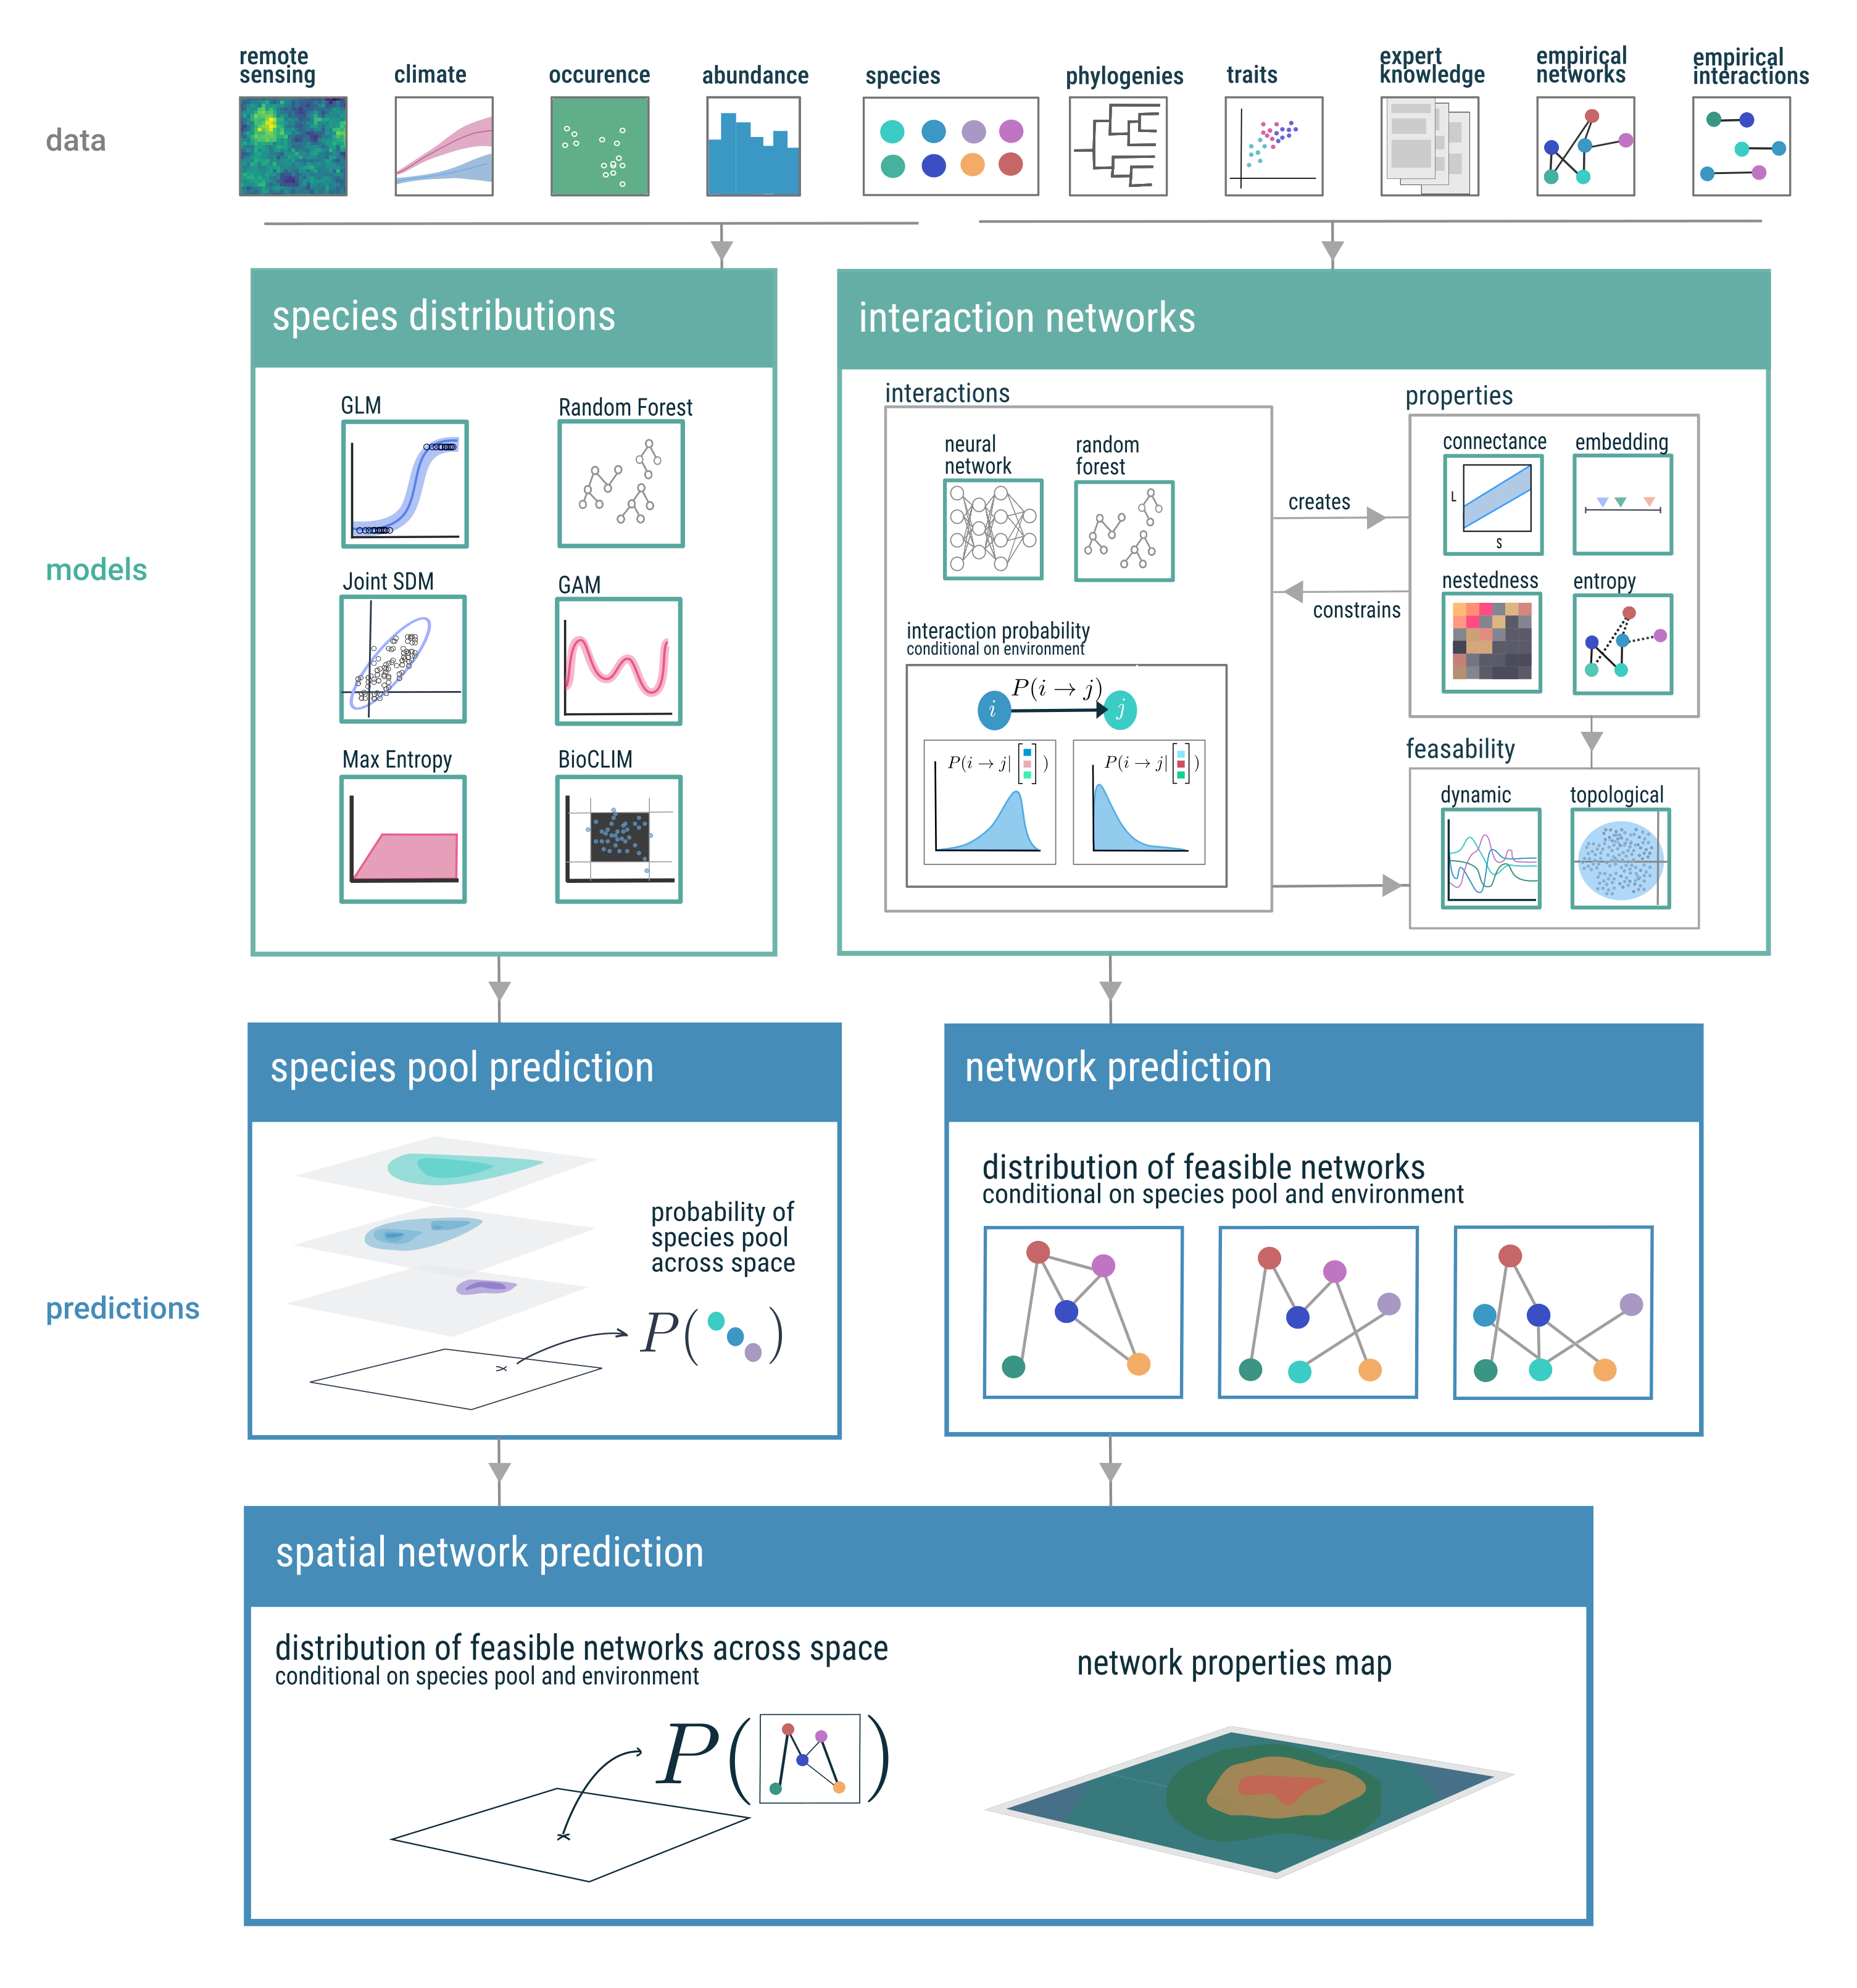
\includegraphics[width=\textwidth]{figures/concept_v6.png}
    \caption{A conceptual roadmap highlighting key areas for the prediction
of ecological networks. Starting with the input of data from multiple
sources, followed by a modelling framework for ecological networks and
the landscape, which are then ultimately combined to allow for the
prediction of spatially explicit networks.}
    \label{fig:conceptual}
\end{figure}

\clearpage

\subsection{Challenges: constraints on
predictions}\label{challenges-constraints-on-predictions}

\subsubsection{Ecological network data are scarce and hard to
obtain}\label{ecological-network-data-are-scarce-and-hard-to-obtain}

At the moment, prediction of species interactions is made difficult by
the limited availability of data. Although we have seen a growth in
species occurrence data, this growth is much slower for ecological
interactions because species interactions are challenging to sample
comprehensively (\cite{Bennett2019PotPit, Jordano2016SamNet}) and
sampling methodology has strong effects on the resulting data
(\cite{deAguiar2019RevBia}). In turn, the difficulty of sampling
interactions can lead to biases in our understanding of network
structure (\cite{deAguiar2019RevBia}). This knowledge gap has motivated a
variety of approaches to deal with interactions in ecological research
based on assumptions that do not always hold, such as the assumption
that co-occurrence is equivalent to meaningful interaction strength
(\cite{Blanchet2020Cooccurrence}). Spatial biases in data coverage are prevalent
at the global scale (with South America, Africa and Asia being
under-represented) and different interaction types show biases towards
different biomes (\cite{Poisot2021GloKno}). These ``spatial gaps'' serve
as a limitation to our ability to confidently make predictions when
accounting for real-world environmental conditions, especially in
environments for which there are no analogous data.

Further, empirical estimation of interaction \emph{strength} is highly
prone to bias as existing data are usually summarised at the taxonomic
scale of the species or higher, thereby losing information that
differentiates the strength in per-individual interactions from the
strength of a whole species interaction (\cite{Wells2013SpeInt}).
Empirical estimations of interaction strength are still crucial
(\cite{Novak2008EstNon}), but are a hard task to quantify in natural
communities (\cite{Wootton1997EstTes, Sala2002ComDis,
Wootton2005MeaInt}), especially as the number of species composing
communities increases, compounded by the possibility of higher-order
interactions or non-linear responses in interactions
(\cite{Wootton2005MeaInt}). Further, interaction strength is often
variable and context dependent and can be influenced by
density-dependence and spatio-temporal variation in community
composition (\cite{Wootton2005MeaInt}).

\subsubsection{Powerful predictive tools work better on large data
volumes}\label{powerful-predictive-tools-work-better-on-large-data-volumes}

This scarcity of data limits the range of computational tools that can
be used by network ecologists. Most deep learning methods, for instance,
are very data expensive. The paucity of data is compounded by a
collection of biases in existing datasets. Species interaction data are
typically dominated by food webs, pollination, and host-parasite
networks (\cite{Ings2009EcoNet, Poisot2020EnvBia}). This could prove to
be a limiting factor when trying to understand or predict networks of
underrepresented interaction types or when trying to integrate networks
of different types (\cite{Fontaine2011EcoEvo}), especially given their
inherent structural variation (\cite{Michalska-Smith2019TelEco}). This
stresses the need for an integrated, flexible, and data-efficient set of
computational tools which will allow us to predict ecological networks
accurately from existing and imperfect datasets, but also enable us to
perform model validation and comparison with more flexibility than
existing tools. We argue that \autoref{fig:example} is an example of the promise
of these tools \emph{even} when facing datasets of small size. The
ability to extract and engineer features also serves to bolster our
predictive power. Although it may be tempting to rely on approaches like
bootstrapping to estimate the consistency of the predictions, we are
confronted with the issues of low data volume and data bias---that we
are more likely to observe interactions between some pairs of species
(\emph{i.e.,} those that co-occur often, e.g. \cite{Cazelles2015TheSpe}, and those
with higher relative abundance, e.g. \cite{Vazquez2009UniPat}). This
introduces risk in training models on pseudo-replicated data. In short,
the current lack of massive datasets must not be an obstacle to
prediction; it is an ideal testing ground to understand how little data
is sufficient to obtain actionable predictions, and how much we can rely
on data inflation procedures to reach this minimal amount.

\subsubsection{Scaling-up predictions requires scaled-up
data}\label{scaling-up-predictions-requires-scaled-up-data}

We are also currently limited by the level of biological organisation at
which we can describe ecological networks. For instance, our
understanding of individual-based networks (\emph{e.g.,} \cite{Araujo2008NetAna,
Tinker2012StrMec}) is still in its infancy (\cite{Guimaraes2020StrEco})
and acts as a resolution-limit. Similarly, the resolution of
environmental (or landscape) data also limits our ability to predict
networks at small scales, although current trends in remote sensing
would suggest that this will become less of a hindrance with time
(\cite{Makiola2020KeyQue}). Ecosystems are a quintessential
complex-adaptive-system (\cite{Levin1998EcoBio}) with a myriad of
processes at different spatial, temporal, and organisational scales that
influence and respond to one another. Understanding how the product of
these different processes drive the properties of ecosystems across
different scales remains a central challenge of ecological research, and
we should strive to work on methods that will integrate different
empirical ``snapshots'' of this larger system.

\subsection{Opportunities: an emerging ecosystem of open tools and
data}\label{opportunities-an-emerging-ecosystem-of-open-tools-and-data}

\subsubsection{Data are becoming more
interoperable}\label{data-are-becoming-more-interoperable}

The acquisition of biodiversity and environmental data has tremendously
increased over the past decades thanks to the rise of citizen science
(\cite{Dickinson2010CitSci}) and of novel technology
(\cite{Stephenson2020TecAdv}), including wireless sensors
(\cite{Porter2005WirSen}), next-generation DNA sequencing
(\cite{Creer2016EcoSF}), and remote sensing (\cite{Skidmore2015AgrBio,
Lausch2016LinEar}). Open access databases, such as
\href{https://www.gbif.org/}{GBIF} (for biodiversity data),
\href{https://www.ncbi.nlm.nih.gov/}{NCBI} (for taxonomic and genomics
data), \href{https://www.treebase.org/treebase-web/home.html}{TreeBASE}
(for phylogenetics data), \href{https://icestes.github.io/}{CESTE}
(\cite{Jeliazkov2020GloDat}) (for metacommunity ecology and species traits
data), and \href{https://www.worldclim.org/data/bioclim.html}{WorldClim}
(for bioclimatic data) contain millions of data points that can be
integrated to monitor and model biodiversity at the global scale. For
species interactions data, at the moment
\href{https://mangal.io/#/}{Mangal} is the most comprehensive open
database of published ecological networks (\cite{Poisot2016ManMak}), and
\href{https://www.globalbioticinteractions.org/about}{GloBI} is an
extensive database of realised and potential species interactions
(\cite{Poelen2014Global}). Developing standard practices in data
integration and quality control (\cite{Kissling2018BuiEss}) and in
next-generation biomonitoring (NGB; \cite{Makiola2020KeyQue}) would
improve our ability to make reliable predictions of ecosystem properties
on increasing spatial and temporal scales. The advancement of prediction
techniques coupled with a movement towards standardising data collection
protocols (e.g. \cite{Perez-Harguindeguy2013NewHan} for plant functional
traits) and metadata (e.g.
\href{https://www.tdwg.org}{DarwinCore})---which facilitates
interoperability and integration of datasets---as well as a growing
interest at the government level (\cite{Scholes2012BuiGlo}) paints a
positive picture for data access and usability in the coming years.

\subsubsection{Machine learning tools are becoming more
accessible}\label{machine-learning-tools-are-becoming-more-accessible}

This effort is also supported by a thriving ecosystem of data sources
and novel tools. ML methods can often be more flexible and perform
better than classical statistical methods, and can achieve a very high
level of accuracy in many predictive and classification tasks in a
relatively short amount of time (e.g., \cite{Cutler2007RanFor,
Krizhevsky2017ImaCla}). Increasing computing power combined with
recent advances in machine learning techniques and applications shows
promise in ecology and environmental science (see \cite{Christin2019AppDee}
for an overview). Moreover, ongoing developments in deep learning are
aimed at improvement in low-data regimes and with unbalanced datasets
(\cite{Antoniou2018DatAug, Chawla2010DatMin}). Considering the current
biases in network ecology (\cite{Poisot2021GloKno}) and the scarcity of
data of species interactions, the prediction of ecological networks will
undoubtedly benefit from these improvements. Machine learning methods
are emerging as the new standard in computational ecology in general
(\cite{Olden2008MacLea, Christin2019AppDee}), and in network ecology in
particular (\cite{Bohan2017NexGlo}), as long as sufficient, relevant data
are available. Many studies have used machine learning models
specifically with ecological interactions. Relevant examples include
species traits used to predict interactions and infer trait-matching
rules (\cite{Desjardins-Proulx2017EcoInt, Pichler2020Machine}), automated
discovery of food webs (\cite{Bohan2011AutDis}), reconstruction of
ecological networks using next-generation sequencing data
(\cite{Bohan2017NexGlo}), and network inference from presence-absence data
(\cite{Sander2017EcoNet}). As many ecological and evolutionary processes
underlie species interactions and the structure of their ecological
networks (\emph{e.g.,} \cite{Vazquez2009UniPat, Segar2020RolEvo}, it can be
difficult to choose relevant variables and model species interactions
networks explicitly. A promising application of machine learning in
natural sciences is Scientific-Machine Learning (SciML), a framework
that combines machine learning with mechanistic models
(\cite{Chuang2018AdvCon, Rackauckas2020UniDif}).

\section{A primer on predicting ecological
networks}\label{a-primer-on-predicting-ecological-networks}

Within the constraints outlined in the previous section, we now provide
a primer on the background concepts necessary to build predictive models
of species interaction networks, with a focus on using machine learning
approaches in the modelling process. As @fig:conceptual illustrates,
this involves a variety of numerical and computational approaches;
therefore, rather than an exhaustive summary, we aim to convey a
high-level understanding that translates the core concepts into their
application to ecological networks.

\subsection{Models}\label{models}

\subsubsection{What is a predictive
model?}\label{what-is-a-predictive-model}

Models are used for many purposes, and the term ``model'' itself
embodies a wide variety of meanings in scientific discourse. All models
can be thought of as a function, \(f\), that takes a set of inputs \(x\)
(also called features, descriptors, or independent variables) and
parameters \(\theta\), and maps them to predicted output states \(y\)
(also called label, response, or dependent variable) based on the input
to the model: \(y=f(x,\theta)\).

A given model \(f\) can be used for either descriptive or predictive
purposes. Many forms of scientific inquiry are based around using models
\emph{descriptively}, a practice also called inference, the inverse
problem, fitting a model, or training a model (\cite{Stouffer2019AllEco}).
In this context, the goal of using a model is to estimate the
parameters, \(\theta\), that best explain a set of empirical
observations, \(\{\hat{x}, \hat{y}\}\). In some cases, these parameter
values are themselves of interest (e.g., the strength of selection,
intrinsic growth rate, dispersal distance), but in others cases, the
goal is to compare a set of competing models \(f_1, f_2, \dots\) to
determine which provides the most parsimonious explanation for a
dataset. The quantitative representation of ``effects'' in these
models---the influence of each input on the output---is often assumed to
be linear, and within the frequentist world-view, the goal is often to
determine if the coefficient corresponding with an input is non-zero to
determine its ``significance'' (often different from its ecological
relevance \cite{Martinez-Abrain2008StaSig}) in influencing the outcome.

Models designed for inference have utility---descriptive models of
networks can reveal underlying mechanisms that structure ecological
communities, given a proper null model (\cite{Connor2017UsiNul}). However,
in order for ecology to develop as a predictive science
(\cite{Evans2012PreEco}), interest has grown in developing models that are
used not just for description of data, but also for prediction.
Predictive models are based in \emph{the forward problem}, where the aim
is to predict new values of the output \(y\) given an input \(x\) and
our estimate value of \(\theta\) (\cite{Stouffer2019AllEco}). Because the
forward problem relies on an estimate of \(\theta\), then, the problem
of inference is nested within the forward problem (\autoref{fig:models}): working
towards a predictive view of ecological networks will give us the needed
tools to further our understanding of them.

\begin{figure}[h]
    \centering
    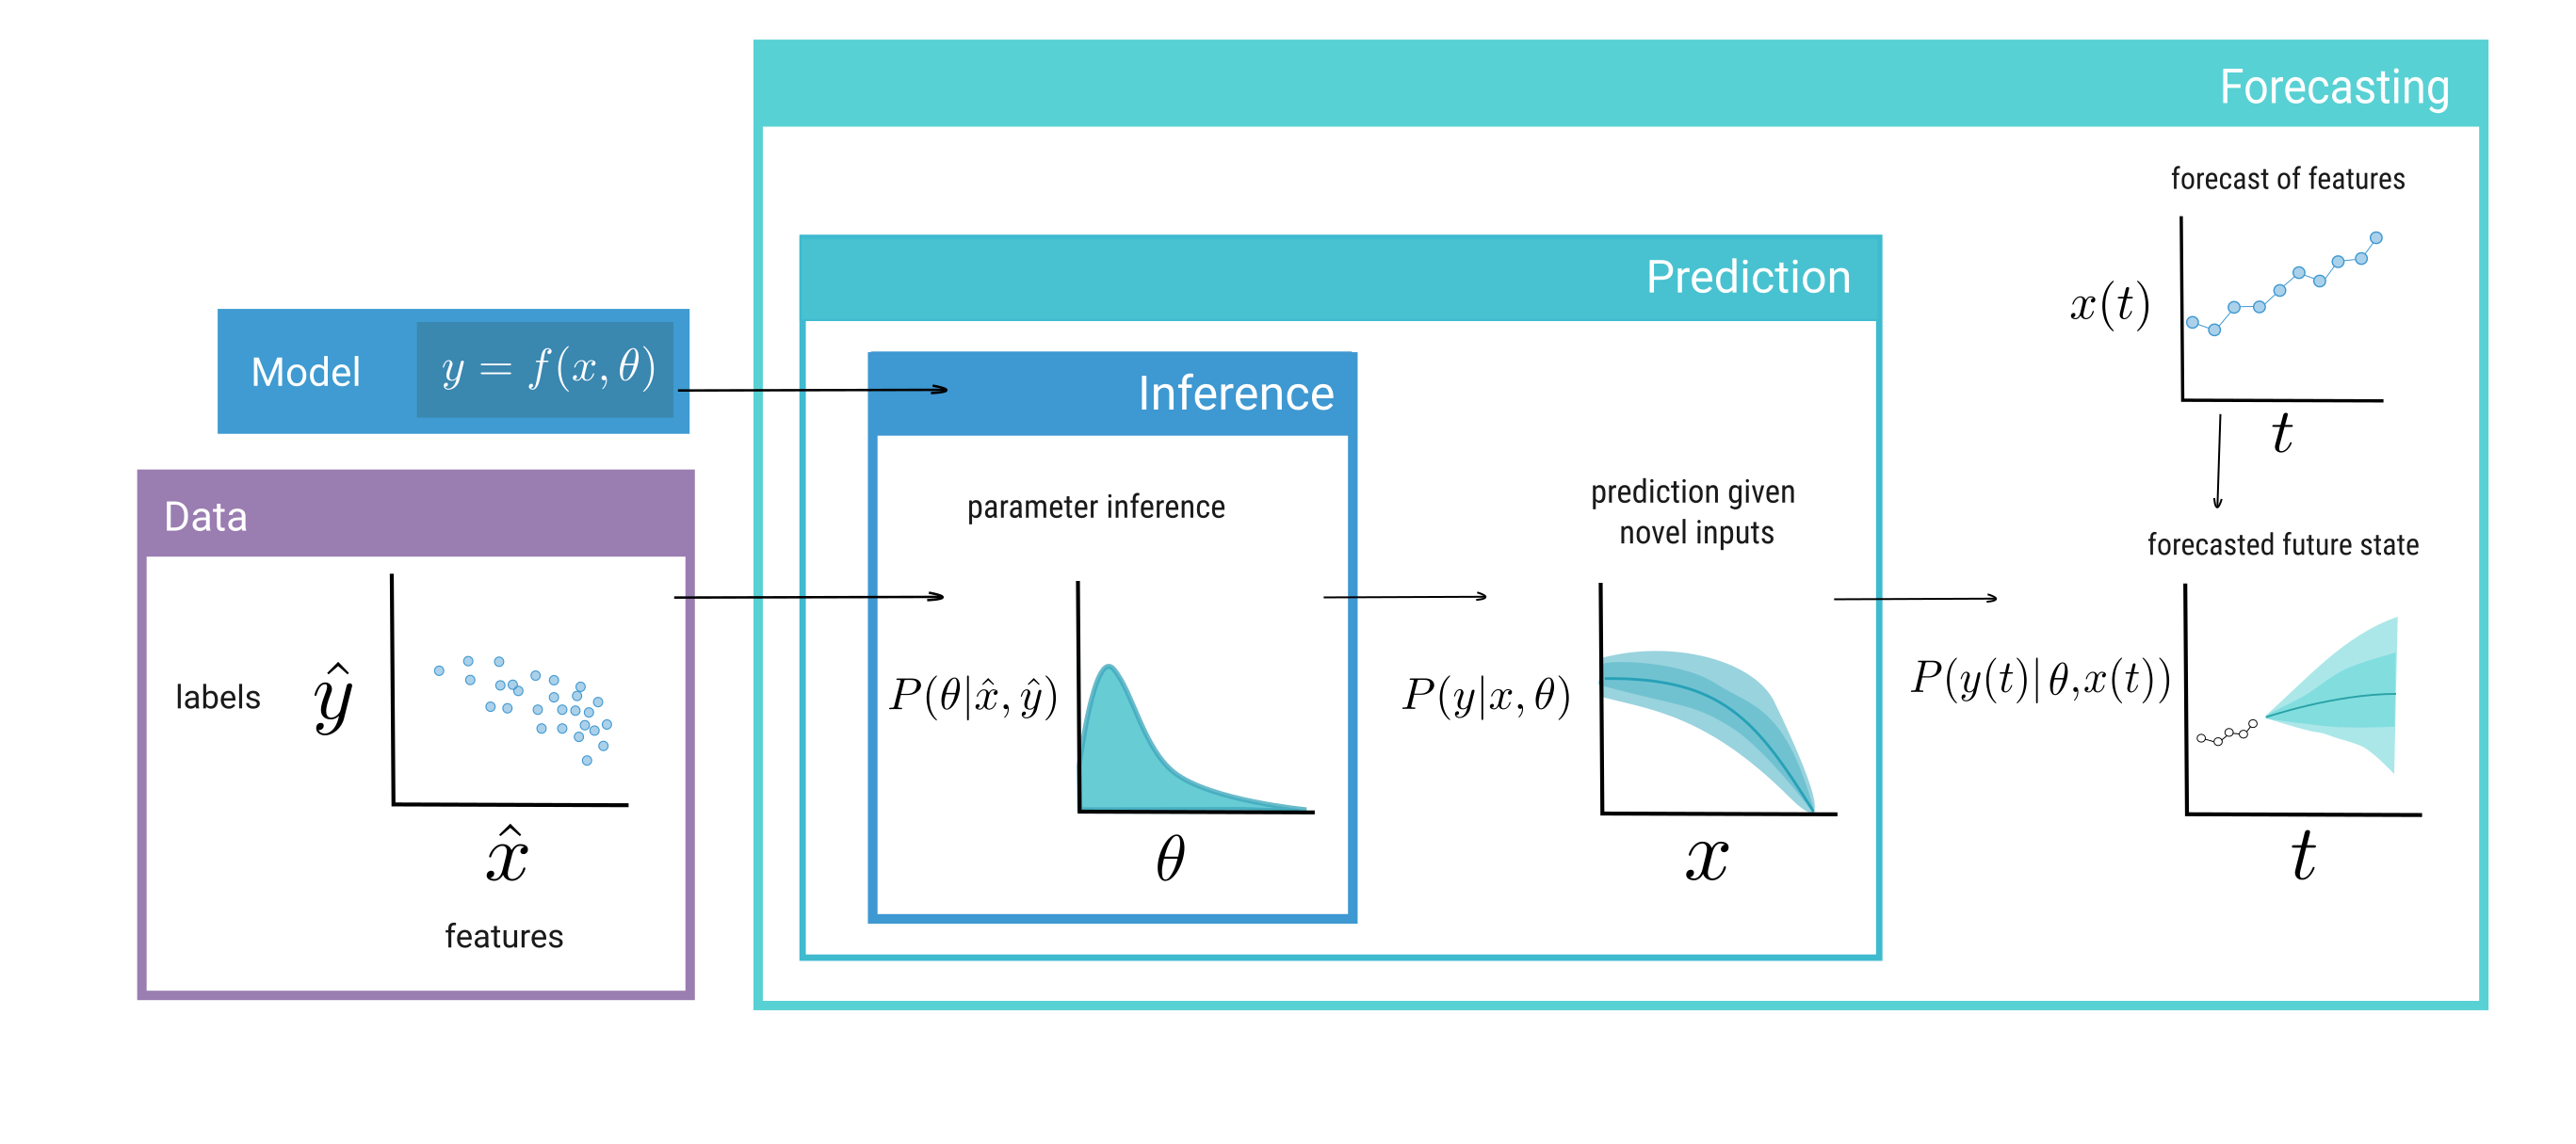
\includegraphics[width=\textwidth]{figures/forecasting_v4.png}
    \caption{The nested nature of developing predictive and forecasting
models, showcases the \emph{forward problem} and how this relies on a
hierarchical structure of the modelling process. The choice of a
specific modelling technique and framework, as well as the data retained
to be part of this model, proceeds directly from our assumptions about
which ecological mechanisms are important in shaping both extant and
future data.}
    \label{fig:models}
\end{figure}

\clearpage

\subsubsection{What do you need to build a predictive
model?}\label{what-do-you-need-to-build-a-predictive-model}

To build a predictive model, one needs the following: first,
\textbf{data}, split into features \(\hat{x}\) and labels \(\hat{y}\)
(@fig:models). Second, a \textbf{model} \(f\), which maps features \(x\)
to labels \(y\) as a function of parameters \(\theta\),
i.e.~\(y = f(x, \theta)\). Third, a \textbf{loss function}
\(L(\hat{y}, y)\), which describes how far a model's prediction \(y\) is
from an empirical value \(\hat{y}\). Lastly, \textbf{priors} on
parameters, \(P(\theta)\), which describe the modeller's \emph{a priori}
belief about the value of the parameters; rather than making an analysis
implicit, specifying priors has the merit of making the modeller's
assumptions explicit, which is a most desirable feature when
communicating predictions to stakeholders
(\cite{Spiegelhalter2000BayMet}). Often an important step before fitting a
model is feature engineering: adjusting and reworking the features to
better uncover feature-label relationships (\cite{Kuhn2019FeaEng}). This
can include projecting the features into a lower dimensional space, as
we did through a probabilistic PCA in the case study, or removing the
covariance structure using a Whitening approach. Then, when a model is
fitted (synonymous with parameter inference or the inverse problem, see
\autoref{fig:models}), a fitting algorithm attempts to estimate the values of
\(\theta\) that minimises the mean value of loss function
\(L(\hat{y},y)\) for all labels \(\hat{y}\) in the provided data \(Y\).
In a Bayesian approach, this typically relys on drawing candidate
parameter values from priors and applying some form of sampling to
generate a posterior estimate of parameters,
\(P(\theta | \hat{x}, \hat{y})\). In the training of neural networks,
this usually involves some form of error back-propagation across the
edges in order to tune their weights, and the biases of each nodes.

\subsubsection{How do we validate a predictive
model?}\label{how-do-we-validate-a-predictive-model}

After we fit a model, we inevitably want to see how ``good'' (meaning,
``fit for purpose'') it is. This process can be divided into two parts:
(i)) model selection, where the modeller chooses from a set of possible
models and (ii) model assessment, where the modeller determines the
performance characteristics of the chosen model (\cite{Hastie2009EleSta}).

In the context of \emph{model selection}, a naïve initial approach is to
simply compute the average error between the model's prediction and the
true data we have, and choose the model with the smallest
error---however this approach inevitably results in \emph{overfitting}.
One approach to avoid overfitting is using information criteria (e.g.,
AIC, BIC, MDL) based around the heuristic that good models maximise the
ratio of information provided by the model to the number of parameters
it has. However, when the intended use-case of a model is prediction the
relevant form of validation is \emph{predictive accuracy}, which should
be tested with \emph{cross-validation}. Cross-validation methods divide
the original dataset into two---one which is used to fit the model
(called the \emph{training} set) and one used to validate its predictive
accuracy on the data that it hasn't ``seen'' yet (called the \emph{test}
set) (\cite{Bishop2006PatRec}). This procedure is often repeated across
different test and training subdivisions of the dataset (either picked
randomly or stratified by some criteria, like balance between positive
and negative interactions in the case study) to determine the
uncertainty associated with our measurement due to our choice of test
and training sets (\cite{Arlot2010SurCro}), in the same conceptual vein as
data bootstrapping: the mean value of the validation metric gives an
overall estimate of its performance, and the variance around this mean
represents the effect of using different data for training and testing.
In a robust model/dataset combination, we expect this variance to be
low, although there are no prescriptive guidelines as to how little
variance is acceptable; the choice of whether to use a model is often
left to the best judgement of the modeller.

We still have to define what \emph{predictive accuracy} means in the
context of interaction network prediction. In the proof-of-concept, we
used a neural-network to perform binary classification by predicting the
presence/absence of an interaction between any two species. There are
two ways for the model to be right: the model predicts an interaction
and there is one (a \emph{true positive} (TP)), or the model predicts no
interaction and there isn't one (a \emph{true negative} (TN)).
Similarly, there are two ways for the model to be wrong: the model
predicts an interaction which does not exist (a \emph{false positive}
(FP)), or the model predicts no interaction but it does exist (a
\emph{false negative} (FN)).

A naïve initial approach to measure how well a model does is
\emph{accuracy}, i.e. the proportion of values it got correct. However,
consider what we know about interaction networks: they are often very
sparse, with connectance usually below a third (\cite{Cohen1990ComFoo}).
If we build a model that always guesses there will be no interaction
between two species, it will be correct in the majority of cases because
the majority of potential interactions in a network typically do not
exist. Therefore this ``empty-matrix'' model would always have an
\emph{accuracy} of \(1-C\), where \(C\) is the observed connectance,
which would almost always be greater than 50\%. Understanding model
performance within sensitivity-specificity space may be more
informative, where sensitivity evaluates how good the model is at
predicting true interactions (True Positive Rate) and specificity refers
to the prediction of true ``non-interactions'' (True Negative Rate). It
must be noted that in ecological networks, there is no guarantee that
the ``non-interactions'' (assumed true negatives) in the original
dataset are indeed true negatives (\cite{Jordano2016ChaEco,
Jordano2016SamNet}). This can result in the positive/negative values,
and the false omission/discovery being artificially worse, and
specifically decrease our confidence in predicted interactions.

In response to the general problem of biases in classifiers, many
metrics have been proposed to measure binary-classifiers
(\cite{Gu2009EvaMea, Drummond2006CosCur}) and are indicative of how well
the model performs with regards to some aspect of accuracy, sensitivity,
specificity and/or precision (\autoref{tbl:validation}). Ultimately the choice of
metric will depend on the intended use of the model: there is not a
single definition of ``success'', but rather different interpretation of
what sources of error are acceptable for a given application.

\begin{table}[h!]
\resizebox{\textwidth}{!}{
\centering
\begin{tabular}{||c c c c||} 
 \hline
 Name & Value & Success & Description \\ [0.2ex] \hline\hline
 Random accuracy & 0.56 & & Fraction of correct predictions if the
classifier is random \\ 
 Accuracy & 0.81 & \(\rightarrow 1\) & Observed fraction of correct
predictions \\
 Balanced accuracy & 0.80 & \(\rightarrow 1\) & Average fraction of
correct positive and negative predictions \\
& & & \\
True Positive Rate & 0.77 & \(\rightarrow 1\) & Fraction of interactions
predicted \\
True Negative Rate & 0.83 & \(\rightarrow 1\) & Fraction of
non-interactions predicted \\
False Positive Rate & 0.16 & \(\rightarrow 0\) & Fraction of
non-interactions predicted as interactions \\
False Negative Rate & 0.22 & \(\rightarrow 0\) & Fraction of
interactions predicted as non-interactions \\
& & & \\
ROC-AUC & 0.86 & \(\rightarrow 1\) & Proximity to a perfect prediction
(ROC-AUC=1) \\
Youden's J & 0.60 & \(\rightarrow 1\) & Informedness of predictions
(trust in individual prediction) \\
Cohen's \(\kappa\) & 0.58 & \(\ge 0.5\) & \\
& & & \\
Positive Predictive Value & 0.66 & \(\rightarrow 1\) & Confidence in
predicted interactions \\
Negative Predictive Value & 0.89 & \(\rightarrow 1\) & Confidence in
predicted non-interactions \\
False Omission Rate & 0.10 & \(\rightarrow 0\) & Expected proportion of
missed interactions \\
False Discovery Rate & 0.33 & \(\rightarrow 0\) & Expected proportion of
wrongly imputed interactions \\ [0.2ex] 
 \hline
\end{tabular}
}
\caption{Overview of the validation statistics applied to the case
study, alongside the criteria indicating a successful classifier and a
guide to interpretation of the values. Taken together, these validation
measures indicate that the model performs well, especially considering
that it is trained from a small volume of data.}
\label{tbl:validation}
\end{table}

In the machine learning literature, a common way of visualising this
extensive list of possible metrics is through the use of ROC
(receiver-operating-characteristic; False Positive Rate on the x-axis,
and True Positive Rate on the y-axis) and PR (precision-recall;
True-Positive-Rate on the x-axis, Positive-predictive-value on the
y-axis) curves (see \autoref{fig:example}). These curves are generated by
considering a continuum of thresholds of classifier acceptance, and
computing the values of ROC/PR metrics for each value of the threshold.
The area-under-the-curve (AUC) is then used as a validation metric and
are typically called AUC-ROC (Area-Under-the-Curve
Receiver-Operator-Curve) and AUC-PR (Area-Under-the-Curve
Precision-Recall) (e.g.~ROC-AUC in Table \ref{tbl:validation}). These measures have
the unstated assumption that the training and testing set are
``correct'', or at least correct enough that the number of true/false
positive/negatives are meaningful; although should this assumption be
true, there would be no need for any predictive approach -- but it is a
well established fact that machine learning systems are resilient to
even relatively high uncertainties in the data (\cite{Halevy2009Unreasonable}).

\subsection{Networks and interactions as predictable
objects}\label{networks-and-interactions-as-predictable-objects}

\subsubsection{Why predict networks and interactions at the same
time?}\label{why-predict-networks-and-interactions-at-the-same-time}

Ecological networks are quite sparse, and larger networks tend to get
sparser (\cite{MacDonald2020Revisiting}); in other words, although networks
are composed of a set of interactions between species pairs, they also
form a much larger set of species pairs that do not interact. If we aim
to predict the structure of networks from the ``bottom-up''--- by
considering each pairwise combination of \(S\) different species---we
are left with \(S^2\) interaction values to estimate, a majority of
which will be 0. Instead, we can use our existing understanding of the
mechanisms that structure ecological networks to whittle down the set of
feasible adjacency matrices, thereby reducing the amount of information
we must predict, and making the problem of predicting interactions less
daunting. The processes that structure ecological networks do not only
occur at the scale of interactions---there are also processes at the
network level which limit what interactions (or how many) are realistic.
The realised structure of a network is the synthesis of the interactions
forming the basis for network structure, and the network structure
refining the possible interactions---``Part makes whole, and whole makes
part'' (\cite{Levins1987DiaBio}).

Another argument for the joint prediction of networks and interactions
is to reduce circularity and biases in the predictions. As an example,
models like linear filtering (\cite{Stock2017LinFil}) generate
probabilities of non-observed interactions existing, but do so based on
measured network properties. Some recent models make interaction-level
predictions (\emph{e.g.,} \cite{Gravel2019Bringing}); these are not unlike stacked
species distribution models, which are individually fit, but
collectively outperformed by joint models or rule-based models
(\cite{Zurell2020TesSpe}). By relying on adequate testing of model
performance of biases (\emph{i.e.,} optimising not only accuracy, but paying
attention to measures like false discovery and false omission rates),
and developing models around a feedback loop between network and
interaction prediction, it is likely that the quality of the predicted
networks will be greatly improved compared to current models.

\subsubsection{What network properties should we use to inform our
predictions of
interactions?}\label{what-network-properties-should-we-use-to-inform-our-predictions-of-interactions}

There are many dimensions of network structure (\cite{Delmas2018Analysing}),
yet there are two arguments to support basing network prediction around
a single property: \emph{connectance} (the ratio of actual edges to
possible edges in the network). First, connectance is ecologically
informative---it relates to resilience to invasion (\cite{Baiser2010ConDet,
Smith-Ramesh2016GloSyn}), can increase robustness to extinction in
food webs (\cite{Dunne2002NetStr}), while decreasing it in mutualistic
networks (\cite{Vieira2015SimSto}), and connectance relates to network
stability (\cite{Landi2018Complexity}). Second, most (if not all) network
properties covary with connectance (\cite{Poisot2014WheEco,
Dunne2002FooStr}).

Within the network science literature, there are numerous methods for
predicting edges based on network properties (\emph{e.g.,} block models
(\cite{Yen2020ComDet}) based on modularity, hierarchical models
(\cite{Kawakatsu2021EmeHie}) based on embedding, etc.). However, in the
context of species interaction networks, these properties often co-vary
with connectance. As a result we suggest that using connectance as the
primary property of interest is most likely to be practical to formulate
at the moment. We have models to estimate species richness over space
(\cite{Jenkins2013GloPat}), and because we can predict connectance from
species richness alone (\cite{MacDonald2020Revisiting}), we can then derive
distributions of network properties from richness estimates, that can
serve to penalise further models that formulate their predictions at the
scale of each possible interaction.

\subsubsection{How do we predict how species that we have never observed
together will
interact?}\label{how-do-we-predict-how-species-that-we-have-never-observed-together-will-interact}

A neutral approach to ecological interactions would assume the
probability of an interaction to mirror the relative abundance of both
species, and would be unaffected by trait variation
(\cite{Poisot2015Species, Pichler2020Machine}); more accurately, a neutral
assumption states that the relative abundances are sufficient to predict
the structure of networks, and this view is rather well supported in
empirical and theoretical systems (\cite{Canard2012EmeStr,
Canard2014EmpEva}). However, functional-trait based proxies could
enable better predictions of ecological interactions
(\cite{Cirtwill2018FeeEnv, Cirtwill2019QuaFra, Bartomeus2016ComFra, Bartomeus2013Understanding}). Selection on functional traits could cause
interactions to be conserved at some evolutionary scales, and therefore
predictions of interaction could be informed by phylogenetic analyses
(\cite{Davies2021EcoRed, Elmasri2020HieBay, Gomez2010EcoInt}).
Phylogenetic matching in bipartite networks is consistent across scales
(\cite{Poisot2018Interactions}), even in the absence of strong selective
pressure (\cite{Coelho2017NeuBio}).

A separate family of methods are based on network embedding (as in the
proof-of-concept). A network embedding projects each node of the network
into a lower-dimensional latent space. Previous explorations of the
dimensionality of food webs have revealed that a reduced number of
dimensions (7) was sufficient to capture most of their structure
(\cite{Eklof2013Dimensionality}); however, recent quantifications of the
complexity of the embedding space of bipartite ecological networks found
a consistent high complexity (\cite{Strydom2021SvdEnt}), suggesting that
the precise depth of embedding required may vary considerably across
systems. Embeddings enables us to represent the structure of a network,
which previously required the \(S^2\) dimensions of an adjacency matrix,
with a smaller number of dimensions. The position of each node in this
lower dimensional space is then treated as a latent measurement
corresponding to the role of that species in the network (\emph{e.g.,}
(\cite{Poisot2021ImpMam}), where a network of about 1500 species was most
accurately described using 12 dimensions). Species close together in
the latent space should interact with similar set of species
(\cite{Rossberg2006FooWeb, Rohr2010ModFoo}). However, these models are
sensitive to sampling biases as they are limited to species for which
there is already interaction data, and as a result a methodological
breakthrough is needed to extend these models to species for which there
is little or no interaction data.

\subsubsection{How do we quantify interaction
strength?}\label{how-do-we-quantify-interaction-strength}

Species interaction networks can also be used as a means to quantify and
understand \emph{interaction strength}. Interaction strength, unlike the
qualitative presence or absence of an interaction, is a continuous
measurement which attempts to quantify the effect of one species on
another. This results in weighted networks representing different
patterns of `flows' between nodes -- which can be modelled in a variety
of ways (\cite{Borrett2019WalPar}). Interaction strength can generally be
divided into two main categories (as suggested by \cite{Berlow2004IntStr}): 1)
the strength of an interaction between individuals of each species, or
2) the effect that changes in one species population has on the dynamics
of the other species. It can be measured as the effect over a period of
time (in the units of biomass or energy flux \cite{Barnes2018EneFlu,
Brown2004MetThe}) or the relative importance of one species on
another (\cite{Heleno2014EcoNet, Berlow2004IntStr, Wootton2005MeaInt}).
One recurring observation is that networks are often composed of many
weak interactions and few strong interactions (\cite{Berlow2004IntStr}).
The distribution of interaction strength within a network effects its
stability (\cite{Neutel2002Stability, Ruiter1995EnePat}) and functioning
(\cite{Duffy2002BioEco, Montoya2003FooWeb}), and serves to benefit
multi-species models (\cite{Wootton2005MeaInt}). Alternatively,
understanding flow in modules within networks can aid in understanding
the organisation of networks (\cite{Farage2021IdeFlo, Montoya2002SmaWor})
or the cascading effects of perturbations (\cite{Gaiarsa2019IntStr}).

In some systems, quantifying interaction strength is relatively
straightforward; this includes a lot of host-parasite systems. For
example, freshwater cyprinid fish can be divided in micro-habitats
(fins, skin, digestive system, gill subsections) and the parasites
counted in each of these micro-habitats, giving within-host resolution
(\cite{Simkova2002AbuRel}); marine sparids and labrids have similarly been
studied this way, see notably (\cite{Sasal1999ComStr,
Desdevises2006DetPar, Morand2002InvPat}). In some cases, within-host
assessments of interaction strengths can reveal macro-ecological events,
like in the conservatism of micro-habitat use in amphibian hosts by
helminths (\cite{Badets2011CorEar}). Even ectoparasites can provide
reliable assessments of interaction strength; for example, when rodent
hosts are minimally disturbed during capture, fine combing of their fur
will result in exhaustive ectoparasites inventories
(\cite{Hadfield2014TalTwo, Karbowiak2019ComImm, Matthee2020DivDis,
Sanchez2014PosCoo, Dickinson2020SamSca}). Parasites have the
desirable property of usually remaining intact within their host during
the interaction, as opposed to prey items as can be recovered through
\emph{e.g.,} gut content analysis or stable isotopes
(\cite{Macias-Hernandez2018MolGut, Schmid-Araya2016TroPos}). As network
ecology is starting to explore the use of predictive models, leading up
to forecasting, we argue that host-parasite systems can provide data
that are reliable and trustworthy enough that they can become the
foundations for methodological development and benchmark studies,
thereby providing more information about host-parasite systems and
supporting the technical development of the field.

Yet in most situations, much like quantifying the occurrence of an
interaction, quantifying interaction \emph{strength} in the field is
challenging in the majority of systems, and one must often rely on
proxies. In some contexts, interaction strength can be estimated via
functional foraging (\cite{Portalier2019MecPre}), where the primary basis
for inferring interaction is foraging behaviour like searching, capture
and handling times. In food-webs, metabolic based models use body mass,
metabolic demands, and energy loss to infer energy fluxes between
organisms (\cite{Yodzis1992BodSiz, Berlow2009SimPre}). In addition,
food-web energetics models can be incorporated at various resolutions
for a specific network, ranging from individual-based data to more
lumped data at the species level or trophic group, depending on data
availability( \cite{Barnes2018EneFlu, Berlow2009SimPre}). Taken together,
these considerations impose too many constraints on predicting
continuous interaction strength at the moment, resulting in our primary
focus in binary present/absent interactions within this manuscript.

\subsubsection{How do we determine what interaction networks are
feasible?}\label{how-do-we-determine-what-interaction-networks-are-feasible}

For several decades, ecologists have aimed to understand how networks of
many interacting species persist through time. The diversity-stability
paradox, first explored by (\cite{May1974StaCom}), shows that under a neutral
set of assumptions ecological networks should become decreasingly stable
as the number of species increases. Yet, in the natural world we observe
networks of interactions that consist of far more species than May's
model predicts (\cite{Albouy2019Marine}). As a result, understanding what
aspects of the neutral assumptions of May's model are incorrect has
branched many investigations into the relationship between ecological
network structure and persistence (\cite{Allesina2012StaCri}). These
assumptions can be split into dynamical assumptions and topological
assumptions. Topologically, we know that ecological networks are not
structured randomly. Some properties, like the aforementioned
connectance, are highly predictable (\cite{MacDonald2020Revisiting}).
Generative models of food-webs (based on network embeddings) fit
empirical networks more effectively than random models
(\cite{Allesina2008GenMod}). These models have long used allometry as a
single-dimensional niche space---naturally we want to extend this to
traits in general. The second approach to stability is through
\emph{dynamics}. Early models of community dynamics rely on the
assumption of linear interaction effects, but in recent years models of
bioenergetic community dynamics have shown promise in basing our
understanding of energy flow in food-webs in the understood relationship
between allometry and metabolism (\cite{Delmas2017SimBio}). An additional
consideration is the multidimensional nature of ``stability'' and
``feasibility'' (\emph{e.g.,} resilience to environmental change vs extinctions; \cite{Dominguez-Garcia2019UnvDim}) and how different disturbances
propagate across levels of biological organisation (\cite{Kefi2019AdvOur,
Gravel2016StaCom}). Recent approaches such as structural stability
(\cite{Saavedra2017StrApp, Ferrera2016EffCom}) allow us to think of
network feasibility in rigorous mathematical terms, which may end up as
usable parameters to penalise network predictions.

\subsubsection{What taxonomic scales are suitable for the prediction of
species
interactions?}\label{what-taxonomic-scales-are-suitable-for-the-prediction-of-species-interactions}

If we use different trait-based proxies to predict potential
interactions between species the choice of such proxies should be
theoretically linked to the taxonomic and spatial scale we are using in
our prediction (\cite{Wiens1989SpaSca}). At some scales we can use
morphological traits of co-occurring species to assess the probability
of interaction between them (\cite{Bartomeus2016ComFra}). On broader
taxonomic scales we can infer interaction probability through the
phylogenetic distance, assuming that functional traits themselves are
conserved (\cite{Gomez2010EcoInt}). In this case, we can think of the
probability that one species will interact with another as the distance
between them in niche-space (\cite{Desjardins-Proulx2017EcoInt}), and this
can be modelled by simulating neutral expectations of trait variation on
phylogenetic trees (\cite{Davies2021EcoRed}). At the narrowest scales, we
may be interested in predicting behavioural traits like foraging
behaviour (\cite{Bartomeus2016ComFra}), and at this scale we may need to
consider abundance's effect on the probability of an encounter
(\cite{Wells2013SpeInt}).

\subsubsection{What about indirect and higher-order
interactions?}\label{what-about-indirect-and-higher-order-interactions}

Although network ecology often assumes that interactions go strictly
from one node to the other, the web of life is made up of a variety of
interactions. Indirect interactions---either higher-order interactions
between species, or interaction strengths that themselves interact ---
have gained interest in recent years( \cite{Golubski2016EcoNet,
Golubski2011ModMod}). One mathematical tool to describe these
situations is hypergraphs: hypergraphs are the generalisation of a
graph, allowing a broad yet manageable approach to complex interactions
(\cite{Carletti2020DynSys}), by allowing for particular interactions to
occur beyond a pair of nodes. An additional degree of complexity is
introduced by multi-layer networks (\cite{Hutchinson2019SeeFor}).
Multi-layer networks include edges across ``variants'' of the networks
(timepoints, locations, or environments). These can be particularly
useful to account for the metacommunity structure
(\cite{Gross2020ModMod}), or to understand how dispersal can inform
conservation action (\cite{Albert2017AppNet}). Ecological networks are
intrinsically multi-layered (\cite{Pilosof2017MulNat}). However,
\emph{prima facie}, increasing the dimensionality of the object we need
to predict (the multiple layers rather than a single network) makes the
problem more complicated. Yet, multi-layer approaches improve prediction
in social networks (\cite{Jalili2017LinPre, Najari2019LinPre,
Yasami2018NovMul}), and they may prove useful in network ecology going
forward.

\subsection{Space}\label{space}

Although networks were initially used to describe the interactions
\emph{within} a community, interest in the last decade has shifted
towards understanding their structure and variation over space
(\cite{Trojelsgaard2016EcoNet, Baiser2019EcoRul}), and has established
network ecology as an important emerging component of biogeography and
macroecology.

\subsubsection{How much do networks vary over
space?}\label{how-much-do-networks-vary-over-space}

Networks can vary across space either in their structural properties
(\emph{e.g.,} connectance or degree distribution) or in their composition
(identity of nodes and edges). Interestingly, variation in the
structural properties of ecological networks primarily responds to
changes in the size of the network. The number of links in ecological
networks scales with the number of species (\cite{MacDonald2020Revisiting, Brose2004Unified}), and connectance and size drive the rest of network
structure (\cite{Poisot2014WheEco, Dunne2002FooStr, Riede2010ScaFoo}).
Species turnover in space results in changes in the composition of
ecological networks. But, this is not the only reason network
composition varies (\cite{Poisot2015Species}). Intraspecific variation can
result in interaction turnovers without changes in species composition
\cite{Bolnick2011WhyInt}. Similarly, changes in species abundances can
lead to variation in interaction strengths (\cite{Canard2014EmpEva,
Vazquez2007SpeAbu}). Variation in the abiotic environment and indirect
interactions \cite{Golubski2016EcoNet} could modify the occurrence and
strength of individual interactions. Despite this, empirical networks
tend to share a common backbone (\cite{BramonMora2018Identifying}) and functional
composition (\cite{Dehling2020SimCom}) across space.

\subsubsection{How do we predict what the species pool at a particular
location
is?}\label{how-do-we-predict-what-the-species-pool-at-a-particular-location-is}

As the species pool forms the basis for network structure, predicting
which species are present at a particular location is essential to
predict networks across space. Species distribution models (SDMs) are
increasingly ubiquitous in macroecology--- these models predict the
range of a species based on known occurrences and environmental
conditions, such as climate and land cover (\cite{Guisan2005PreSpe,
Elith2006NovMet}). Including interactions or co-occurrences in SDMs
generally improves predictive performance (\cite{Wisz2013RolBio}). Several
approaches exist to combine multiple SDMs: community assemblage at a
particular site can be predicted either by combining independent
single-species SDMs (stacked-SDMs, SSDMs) or by directly modelling the
entire species assemblage and multiple species at the same time (joint
SDMs, JSDMs) (\cite{Norberg2019ComEva}). Building on the JSDM framework,
hierarchical modelling of species communities
(\cite{Ovaskainen2017HowMak}) has the advantage of capturing processes
that structure communities. Spatially Explicit Species Assemblage
Modelling (SESAM) constrains SDM predictions using macro-ecological
models (\cite{Guisan2011SesNew}) --- for example, variation in species
richness across space can constrain assemblage predictions
(\cite{DAmen2015UsiSpe}).

The next step is to constrain distribution predictions using network
properties. This builds on previous calls to adopt a probabilistic view:
a probabilistic species pool (\cite{Karger2016DelPro}), and probabilistic
interactions through Bayesian networks (\cite{Staniczenko2017LinMac}).
\cite{Blanchet2020Cooccurrence} argue that the probabilistic view avoids confusion
between interactions and co-occurrences, but that it requires prior
knowledge of interactions. This could potentially be solved through our
framework of predicting networks first, interactions next, and finally
the realised species pool.

\subsubsection{How do we combine spatial and network
predictions?}\label{how-do-we-combine-spatial-and-network-predictions}

In order to predict networks across space, we need to combine multiple
models---one which predicts what the species pool will be at a given
location, and one to predict what interaction networks composed from
this species pool are likely to be (see \autoref{fig:conceptual}). Both of these
models contain uncertainty, and when we combine them the uncertainty
from each model should be propagated into the combined model. The
Bayesian paradigm provides a convenient solution to this---if we have a
chain of models where each model feeds into the next, we can sample from
the posterior of the input models. A different approach is
\emph{ensemble modelling} which combines the predictions made by several
models, where each model is predicting the same thing
(\cite{Parker2013EnsMod}). Error propagation, an important step in
building any ecological model, describes the effect of the uncertainty
of input variables on the uncertainty of output variables
(\cite{Draper1995AssPro, Parysow2000EffApp}). \cite{Benke2018ErrPro} identifies
two broad approaches to model error propagation: analytically using
differential equations or stochastically using Monte-Carlo simulation
methods. Errors induced by the spatial or temporal extrapolation of data
also need to be taken into account when estimating the uncertainty of a
model's output (\cite{Peters2004StrEco}).

\subsection{Time}\label{time}

\subsubsection{Why should we forecast species interaction
networks?}\label{why-should-we-forecast-species-interaction-networks}

Forecasting species interactions are critical for informing ecosystem
management (\cite{Harvey2017BriEco}) and systematic conservation
prioritisation (\cite{Pollock2020ProBio}), and for anticipating
extinctions and their consequences (\cite{McDonald-Madden2016UsiFoo,
McWilliams2019StaMul}). Ecological interactions shape species
distributions at both local and broad spatial scales, and including
interactions in SDM models typically improves predictive performance
(\cite{Araujo2007ImpBio, Wisz2013RolBio, Pigot2013SpeInt}). However,
these tend to rely on approaches involving estimating pairwise
dependencies based on co-occurrence, using surrogates for
biotic-interaction gradients, and hybridising SDMs with dynamic models
(\cite{Wisz2013RolBio}). Most existing models to predict the future
distribution of species ignore interactions (\cite{Urban2016ImpFor}).
Changes in species ranges and phenology will inevitably create
spatiotemporal mismatches and affect encounter rates between species
(\cite{Gilman2010FraCom}), which will further shift the distribution of
species across space. New interactions will also appear between species
that are not currently co-occurring (\cite{Gilman2010FraCom}). Only by
forecasting how species will interact can we hope to have an accurate
portrait of how biodiversity will be distributed under the future
climate.

Forecasting how climate change will alter biodiversity is also crucial
for maximising conservation outcomes. Improving SDMs through
interactions is crucial for conservation, as nearly 30\% of models in
SDM studies are used to assess population declines or landscape ability
to support populations (\cite{Araujo2019StaDis}). Reliable predictions
about how ecological networks will change over time will give us
critical information that could be communicated to decision-makers and
the scientific community about what future environmental risks we are
awaiting and how to mitigate them (\cite{Kindsvater2018OveDat}). Not only
this, but how biodiversity is structured influences the functioning of
the whole ecosystem, community stability and persistence
(\cite{Thompson2012FooWeb, Stouffer2010UndFoo}). Will climate change
impact the distribution of network properties (\emph{e.g.,} connectance)? If so,
which regions or species groups need special conservation efforts? These
overarching questions are yet to be answered (but see
\cite{Albouy2013ProCli, Kortsch2015CliCha, Hattab2016ForFin}). We believe
that the path toward forecasting ecological networks provides useful
guidelines to ultimately better predict how climate change will affect
the different dimensions of biodiversity and ecosystem functioning.

\subsubsection{How do we turn a predictive model into a forecasting
model?}\label{how-do-we-turn-a-predictive-model-into-a-forecasting-model}

On some scales, empirical time-series encode enough information about
ecological processes for machine-learning approaches to make accurate
forecasts. However, there is an intrinsic limit to the predictability of
ecological time-series (\cite{Pennekamp2019IntPre}). A forecast inherently
has a \emph{resolution limit} in space, time, and organisation. For
example, one could never hope to predict the precise abundance of every
species on Earth on every day hundreds of years into the future. There
is often a trade-off between the resolution and horizon of forecast,
\emph{e.g.,} a lower resolution forecast, like primary production will be at a
maximum in the summer, is likely to be true much further into the future
than a higher resolution forecast. If we want to forecast the structure
of ecological networks beyond the forecasting horizon of time-series
based methods, we need forecasts of our predictive model's inputs---a
forecast of the distribution of both environmental conditions and the
potential species pool across space (\autoref{fig:models}).

\subsubsection{How can we validate a forecasting
model?}\label{how-can-we-validate-a-forecasting-model}

Often the purpose of building a forecasting model is to inform
\emph{present} action (\cite{Dietze2018IteNea}). Yet, the nature of
forecasting---trying to predict the future---is that you can only know
if a forecast is ``right'' once it is too late to change it. If we want
to maximise the chance that reality falls within a forecasting model's
predictions, there are two directions to approach this problem: the
first is to extend model validation techniques to a forecasting context,
and the second is to attempt to maximise the amount of uncertainty in
the forecast without compromising its resolution. Cross-validation (see
\autoref{how-do-we-validate-a-predictive-model}) can be used to test the
efficacy of a forecasting model. Given a time-series of \(N\)
observations, a model can iteratively be trained on the first \(n\)
time-points of data, and the forecasting model's accuracy can be
evaluated on the remaining time-points it hasn't ``seen''
(\cite{Bishop2006PatRec}). This enables us to understand both how much
temporal data is required for a model to be robust, and also enables us
to explore the \emph{forecasting horizon} of a process. Further, this
approach can also be applied in the opposite temporal direction--- if we
have reliable data from the past, ``hindcasting'' can also be used to
test a forecast's robustness.

However, these methods inevitably bump into a hard-limitation on what is
feasible for a forecasting model. The future is uncertain. Any empirical
time-series we use to validate a model was collected in past conditions
that may not persist into the future. Any system we wish to forecast
will undergo only one of many possible scenarios, yet we can only
observe the realised outcome of the system under the scenario that
actually unfolds. It is therefore impossible to assess the quality of a
forecasting model in scenarios that remain hypothetical. If the goal is
to maximise the probability that reality will fall within the forecast's
estimates, forecasts should incorporate as much uncertainty about the
future scenario as possible---one way to do this is ensemble modelling
(\cite{Parker2013EnsMod}). However, as we increase the amount of
uncertainty we incorporate into a forecasting model, the resolution of
the forecast's predictions could shrink (\cite{Lei2017EvaTra}), and
therefore the modeller should be mindful of the trade-off between
resolution and accuracy when developing any forecast. Finally, ensemble
models are not guaranteed to give more accurate results: for example,
\cite{Becker2020PreWil} noted that the ensemble model outperforms the
best-in-class models, which should be taken as an indication that
careful model building and selection is of the utmost importance when
dealing with a problem as complex as the prediction of species
interactions.

\section{Conclusion: why should we predict species interaction
networks?}\label{conclusion-why-should-we-predict-species-interaction-networks}

Because we almost can, and because we definitely should.

A better understanding of species interactions, and the networks they
form, would help unify the fields of community, network, and spatial
ecology; improve the quantification of the functional relationships
between species (\cite{Dehling2018BriElt, OConnor2020Unveiling});
re-evaluate metacommunities in light of network structure
(\cite{Guzman2019MulExt}); and enable a new line of research into the
biogeography of species interactions (\cite{Massol2017ChaFou,
Braga2019Spatial}) which incorporates a synthesis of both Eltonian and
Grinnellian niche (\cite{Gravel2019Bringing}). Further, the ability to
reliably predict and forecast species interactions would inform
conservation efforts for protecting species, communities, and
ecosystems. Integration of species interactions into the assessment of
vulnerability to climate change is a needed methodological advancement
(\cite{Foden2016IucSsc}). International panels draw on models to establish
scientific consensus (\cite{Araujo2019StaDis}), and they can be improved
through more effective prediction of species distributions and
interactions (\cite{Syfert2014UsiSpe}). Further, recent studies argue for
a shift in focus from species to interaction networks for biodiversity
conservation to better understand ecosystem processes
(\cite{Harvey2017BriEco}).

We should invest in network prediction because the right conditions to
do so reliably and rapidly are beginning to emerge. Given the possible
benefits to a variety of ecological disciplines that would result from
an increased ability to predict networks, we feel strongly that the
research agenda we outline here should be picked up by the community.
Although novel technologies are bringing massive amounts of data to some
parts of ecology (primarily environmental DNA and remote sensing, but
now more commonly image analysis and bioacoustics), it is even more
important to be intentional about \emph{reconciling} data. This involves
not only the work of understanding the processes encoded within data,
but also the groundwork of developing pipelines to bridge the
ever-expanding gap between ``high-throughput'' and ``low-throughput''
sampling methods. An overall increase in the volume of data will not
result in an increase of our predictive capacity as long as this data
increase is limited to specific aspects of the problem. In the areas we
highlight in \autoref{fig:conceptual}, many data steps are still limiting:
documenting empirical interactions is natural history work that doesn't
lend itself to systematic automation; expert knowledge is by design a
social process that may be slightly accelerated by text mining and
natural language processing (but is not yet, or not routinely or at
scale). These limitations are affecting our ability to reconstruct
networks.

But the tools to which we feed these data, incomplete as they may be,
are gradually getting better; that is, they can do predictions faster,
they handle uncertainty and propagate it well, and they can accommodate
data volumes that are lower than we may expect (\cite{Pichler2020Machine}).
It is clear attempting to predict the structure of ecological networks
at any scale is a methodological and ecological challenge; yet it will
result in qualitative changes in our understanding of complex adaptive
systems, as well as changes to our ability to leverage information about
network structure for conservation decision. It is perhaps even more
important to forecast the structure of ecological networks because it is
commonly neglected as a facet of biodiversity that can (and should) be
managed. In fact, none of the Aichi targets mention biostructure or its
protection, despite this being recognised as an important task
(\cite{McCann2007Protecting}), either implicitly or explicitly. Being able to
generate reliable datasets on networks in space or time will make this
information more actionable.

\textbf{Acknowledgements:} We acknowledge that this study was conducted
on land within the traditional unceded territory of the Saint Lawrence
Iroquoian, Anishinabewaki, Mohawk, Huron-Wendat, and Omàmiwininiwak
nations. TS, NF, TP are funded by a donation from the Courtois
Foundation; FB, NF, and TP are funded by IVADO; BM is funded by the
NSERC Alexander Graham Bell Canada Graduate Scholarship and the FRQNT
master's scholarship; FB, GD, NF, and GH are funded by the NSERC
BIOS\(^2\) CREATE program; GD is funded by the FRQNT doctoral
scholarship; DC, TS, LP, and TP are funded by the Canadian Institute of
Ecology \& Evolution; this research was enabled in part by support
provided by Calcul Québec (www.calculquebec.ca) and Compute Canada
(www.computecanada.ca). This work was supported by funding to the Viral
Emergence Research Initiative (VERENA) consortium including NSF BII
2021909. AG and MDC are supported in part by the Liber Ero Chair.

\printbibliography{}
\end{refsection}

\endinput
%%
%% End of file `article1.tex'.
